\documentclass[problem]{mcs}

\begin{pcomments}
  \pcomment{CP_covering_edges}
  \pcomment{from: S09.cp7r. S07.cp7r}
  \pcomment{completely revised from seriously buggy version by ARM 10/21/09}
\end{pcomments}

\pkeywords{
  relations
  digraphs
  covering_edges
  transitive_closure
  DAGs
  positive_path_relation
}

%%%%%%%%%%%%%%%%%%%%%%%%%%%%%%%%%%%%%%%%%%%%%%%%%%%%%%%%%%%%%%%%%%%%%
% Problem starts here
%%%%%%%%%%%%%%%%%%%%%%%%%%%%%%%%%%%%%%%%%%%%%%%%%%%%%%%%%%%%%%%%%%%%%

\begin{problem}
If $a$ and $b$ are distinct nodes of a digraph, then $a$ is said to
\term{cover} $b$ if there is an edge from $a$ to $b$ and every path from
$a$ to $b$ traverses this edge.  If $a$ covers $b$, the edge from $a$ to
$b$ is called a \term{covering edge}.

\bparts

\ppart What are the covering edges in the DAG in Figure~\ref{coverdag}?

% \begin{figure}[h]
% \caption[height=3in]{div-dag}
% \end{figure}

\begin{solution}
TBA
\end{solution}

\newcommand{\covering}[1]{\text{covering}\paren{#1}}

\ppart\label{cover-ok} Let $\covering{D}$ be the subgraph of $D$
consisting of only the covering edges.  Suppose $D$ is a finite \idx{DAG}.
Explain why $\covering{D}$ has the same positive path relation as $D$.

\hint Consider \emph{longest} paths between a pair of vertices.

\begin{solution}
What we need to show is that if there is a path in $D$ between
vertices $a \neq b$, then there is a path consisting only of covering
edges from $a$ to $b$.  But since $D$ is a finite DAG, there must be a
\emph{longest} path from $a$ to $b$.  Now every edge on this path must be a
covering edge or it could be replaced by a path of length 2 or more,
yielding a longer path from $a$ to $b$.
\end{solution}

\ppart\label{+path=} Show that if two \emph{DAG}'s have the same positive
path relation, then they have the same set of covering edges.

\begin{solution}
\begin{proof}

Suppose $C$ and $D$ are DAG's with the same positive path relation and
that $\diredge{a}{b}$ is a covering edge of $C$.  We want to show that
$\diredge{a}{b}$ must also be a covering edge of $D$.

Since $\diredge{a}{b}$ itself defines a (length one) positive length
path in $C$, there must be a positive length path in $D$ from $a$ to
$b$.  If this positive length path in $D$ is of length greater than one,
then the path must consist of a positive length path from $a$ to $c$
followed by a positive length path from $c$ to $b$ for some vertex, $c$.
Also, since $D$ is a DAG, $c$ cannot be $a$ or $b$.

This means there must also be positive length paths in $C$ from $a$ to $c$
and from $c$ to $b$, and neither of these paths can traverse
$\diredge{a}{b}$ or there would be a cycle.  Hence the path from $a$ to
$c$ to $b$ is a path in $C$ that does not traverse $\diredge{a}{b}$,
contradicting the fact that $\diredge{a}{b}$ is a covering edge of $C$.

In sum, there is a length one path from $a$ to $b$ in $D$, namely
$\diredge{a}{b}$, and this is the \emph{only} path from $a$ to $b$ in $D$,
which proves that $\diredge{a}{b}$ is a covering edge in $D$.
\end{proof}

\end{solution}

\ppart Conclude that $\covering{D}$ is the \emph{unique} DAG with the smallest
number of edges among all digraphs with the same positive path relation as
$D$.

\begin{solution}
  By part~\eqref{+path=}, any DAG with the same positive path relation as
  $D$ must contain all the edges of $\covering{D}$.  By part~\eqref{cover-ok},
  $\covering{D}$ has this same positive path relation.  It follows
  immediately that $\covering{D}$ is the unique minimum-size DAG with the
  same positive path relation as $D$.
\end{solution}

\iffalse
\ppart Show that the previous result is not true in general infinite
DAG's.

\hint Consider the DAG for the path-total order on the rational numbers.

\begin{solution}
In the DAG for $<$ on the $\rationals$, there are no covering
edges, so $\widehat{<}$ has no edges.
\end{solution}
\fi
\eparts

The following examples show that the above results
don't work in general for digraphs with cycles.

\begin{staffnotes}
Tell students to skip these last two parts until they have done the
remaining problems.
\end{staffnotes}

\bparts

\ppart\label{12pospath} Describe two graphs with vertices $\set{1,2}$
which have the same set of covering edges, but not the same positive path
relation (\hint Self-loops.)

\begin{solution}
  Let one graph have edges $\set{(1,2), (1,1)}$ and the other
  $\set{(1,2),(2,2)}$.  They have the same set of covering edges, namely,
  $(1,2)$.  But in the second there is a positive length path from 2 to 2,
  namely a path of length one but there is no positive length path from 2
  to 2 in the first graph.
\end{solution}

\ppart\label{cycle-coveringedges}

\renewcommand{\theenumi}{\roman{enumi}}
\renewcommand{\labelenumi}{(\theenumi)}

\begin{enumerate}

\item The \term{complete digraph} without self-loops on vertices
  $1,2,3$ has edges between every two distinct vertices.  What are
  its covering edges?

\item What are the covering edges of the graph with vertices $1,2,3$ and
  edges $\diredge{1}{2}, \diredge{2}{3}, \diredge{3}{1}$?

\item What about their positive path relations?

\end{enumerate}

\begin{solution}
\begin{enumerate}

\item There are no covering edges, since there is always a length two path from
 $a$ to $b$ that does not use the edge $\diredge{a}{b}$.

\item  All three edges are the covering edges.

\item They have the same positive path relation, namely, each vertex is
  connected to all the vertices, including itself, by positive length
  paths.

\end{enumerate}
\end{solution}


\eparts

\begin{figure}
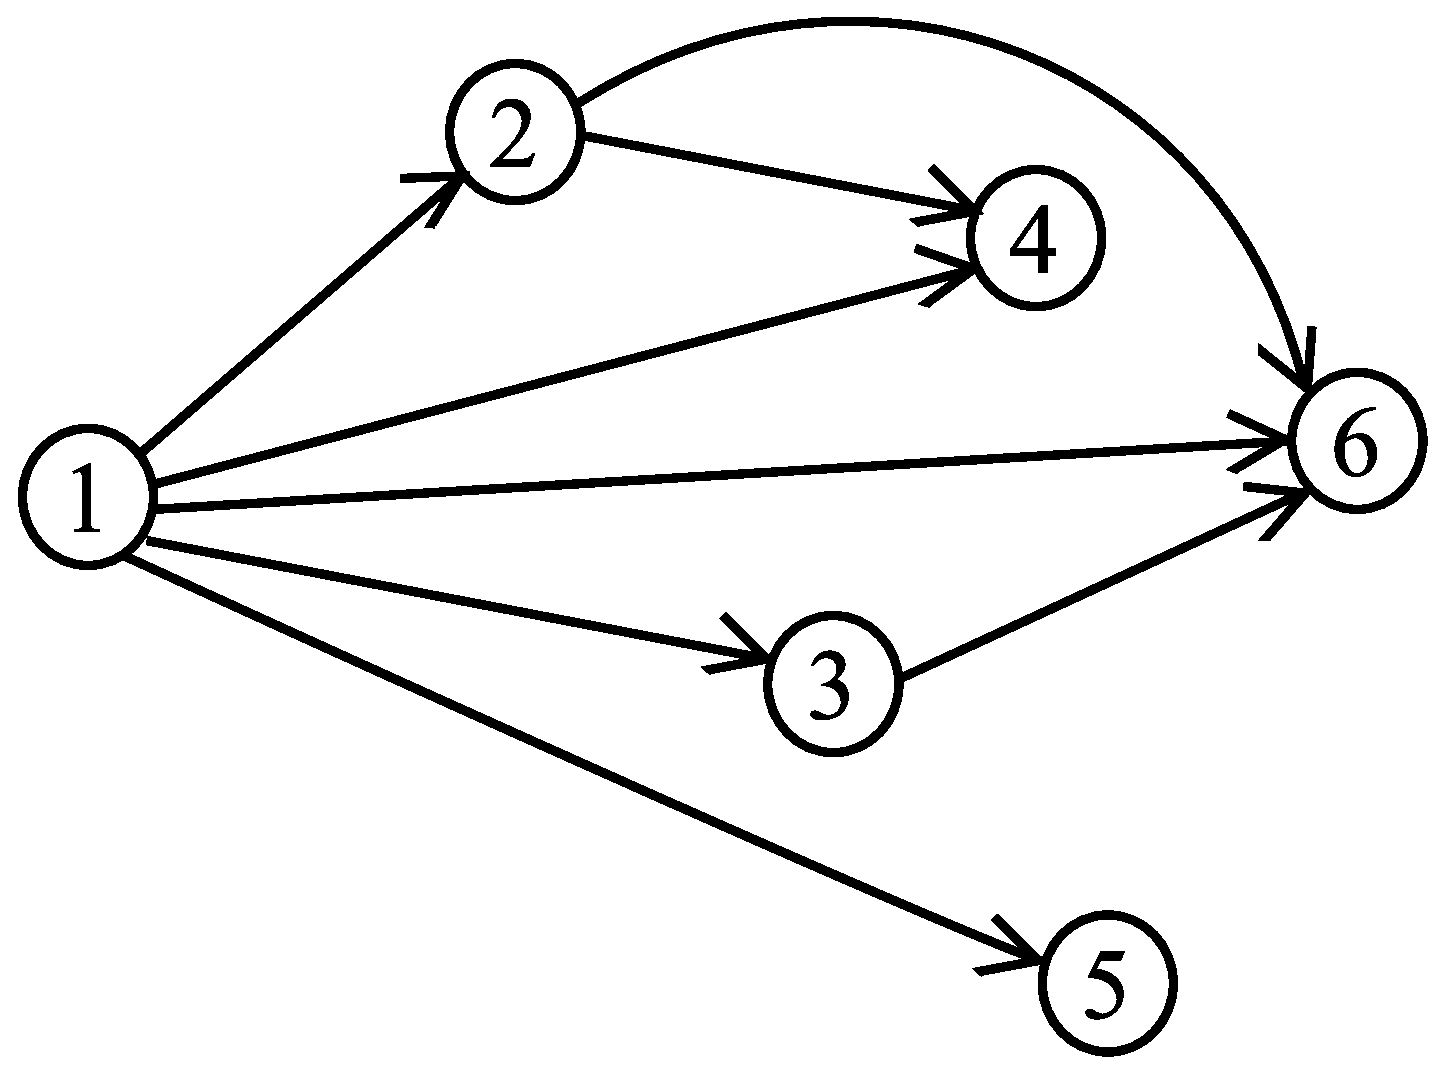
\includegraphics[width = 3in]{div-dag}
\caption{DAG with edges not needed in paths}

\label{coverdag}
\end{figure}

\end{problem}

%%%%%%%%%%%%%%%%%%%%%%%%%%%%%%%%%%%%%%%%%%%%%%%%%%%%%%%%%%%%%%%%%%%%%
% Problem ends here
%%%%%%%%%%%%%%%%%%%%%%%%%%%%%%%%%%%%%%%%%%%%%%%%%%%%%%%%%%%%%%%%%%%%%

\iffalse
Let $D$ be a finite Directed Acyclic Graph (\idx{DAG}).

\bparts

\ppart Explain in one (maybe two) sentences why the \idx{positive path
  relation} of $D$ is obviously a strict partial order.

\begin{solution}
Since following a path from $x$ to $y$ and then a path from $y$ to $z$ is
itself a path from $x$ to $z$, transitivity of the path relation (positive
or not) is immediate.  Also, a path from $x$ to $y$ combined with a path
from $y$ to $x$ would be a cycle, so if a graph is acyclic, its path
relation must be asymmetrical.
\end{solution}

\eparts
\fi
